\chapter[Results for $\Htautau$][Results for $\Htautau$]{Results for $\Htautau$}
\label{chap:results}

\begin{quote}
Results of the $\Htautau$ analysis are described.
\end{quote}

\section{Predictions in the signal region}
\label{sec:results-prefit}

\section{$\Htautauhh$ and $\Htautaull$}
\label{sec:results-hhll}

\section{Fit results}
\label{sec:results-fit}

\clearpage

\begin{figure}[tp]
  \centering
  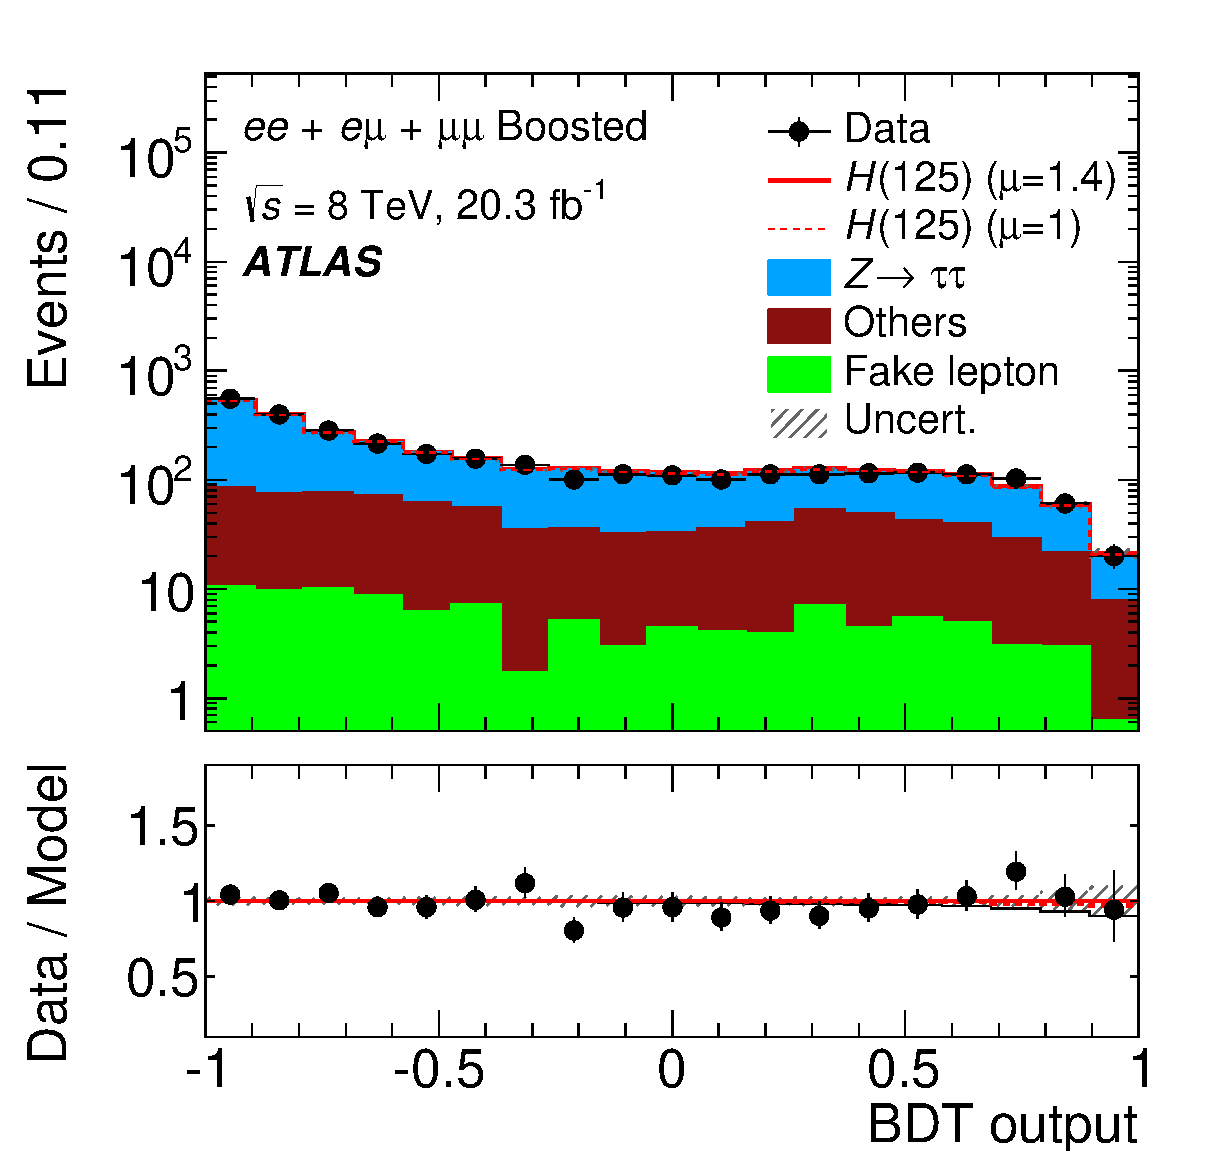
\includegraphics[width=0.48\textwidth]{figures/HIGG-2013-32/fig_08b}
  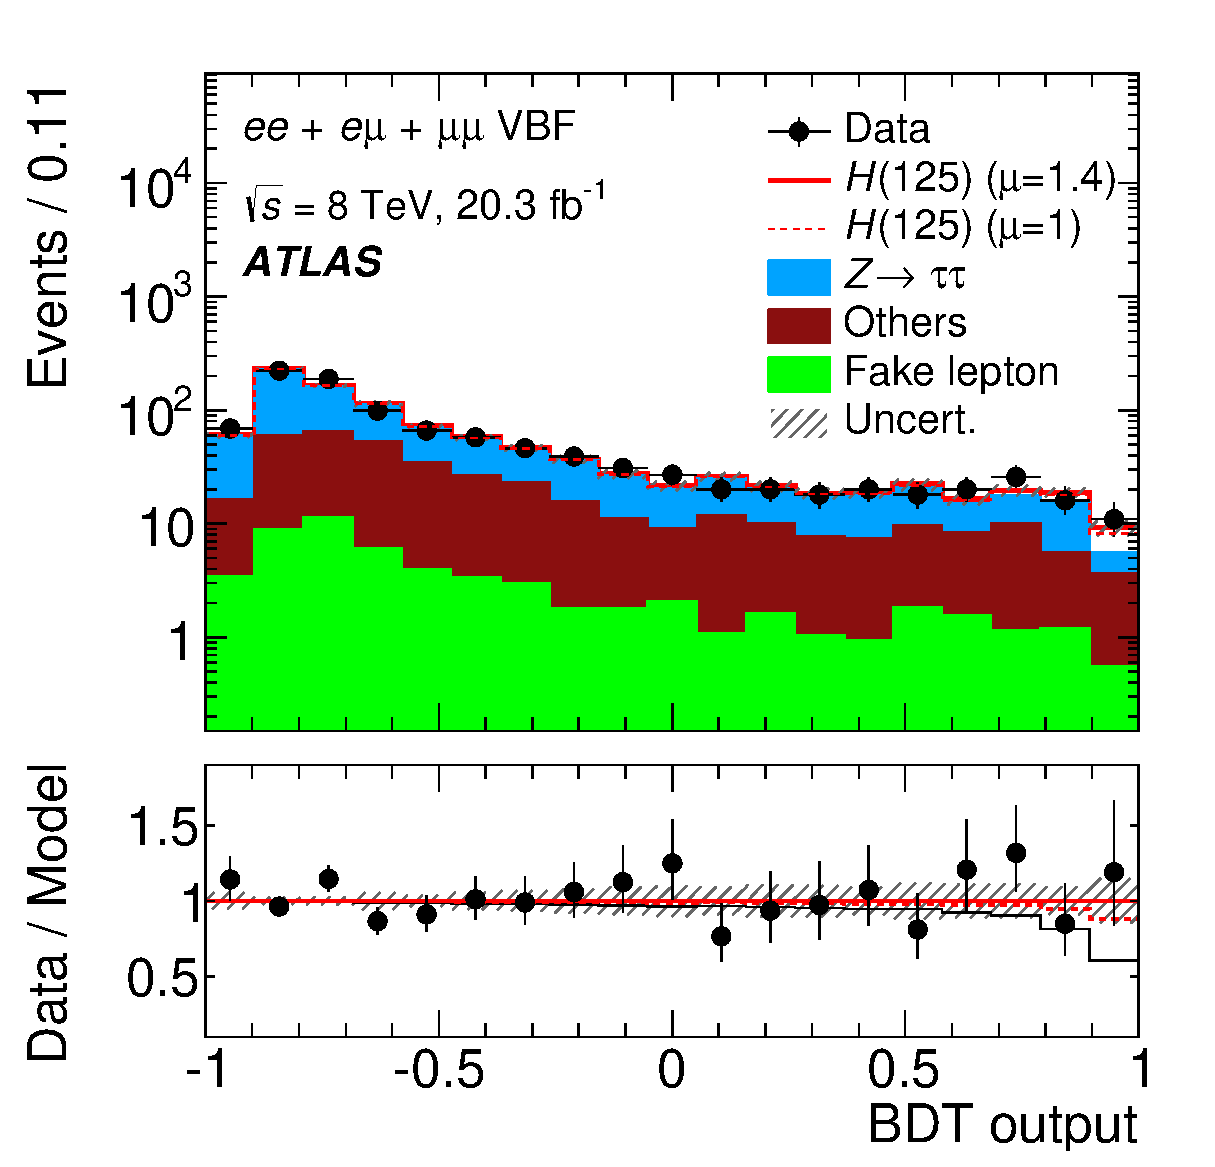
\includegraphics[width=0.48\textwidth]{figures/HIGG-2013-32/fig_08a}
  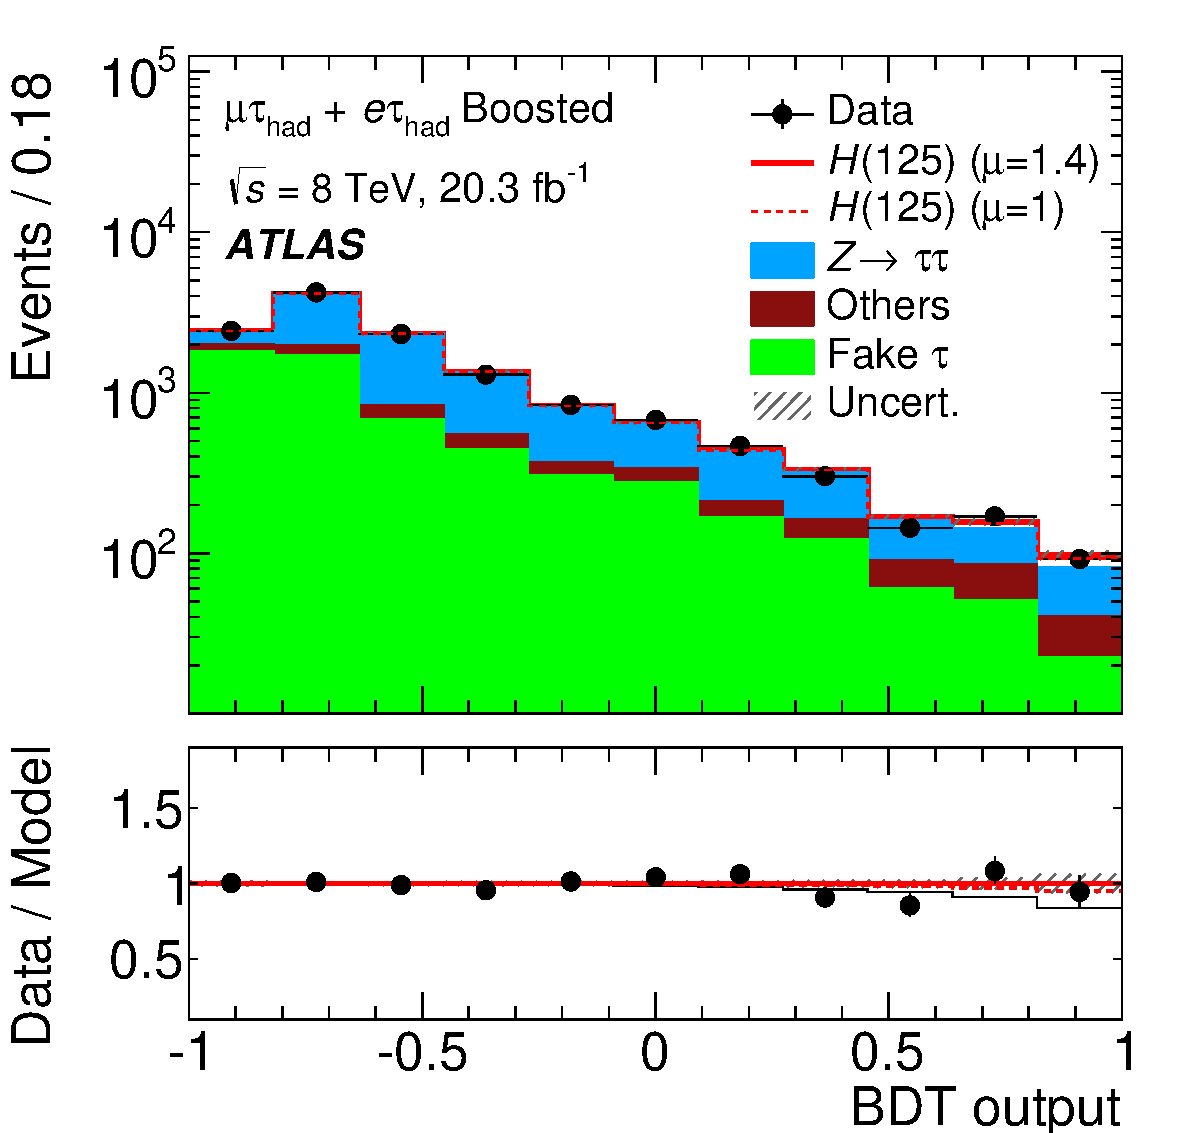
\includegraphics[width=0.48\textwidth]{figures/HIGG-2013-32/fig_08d}
  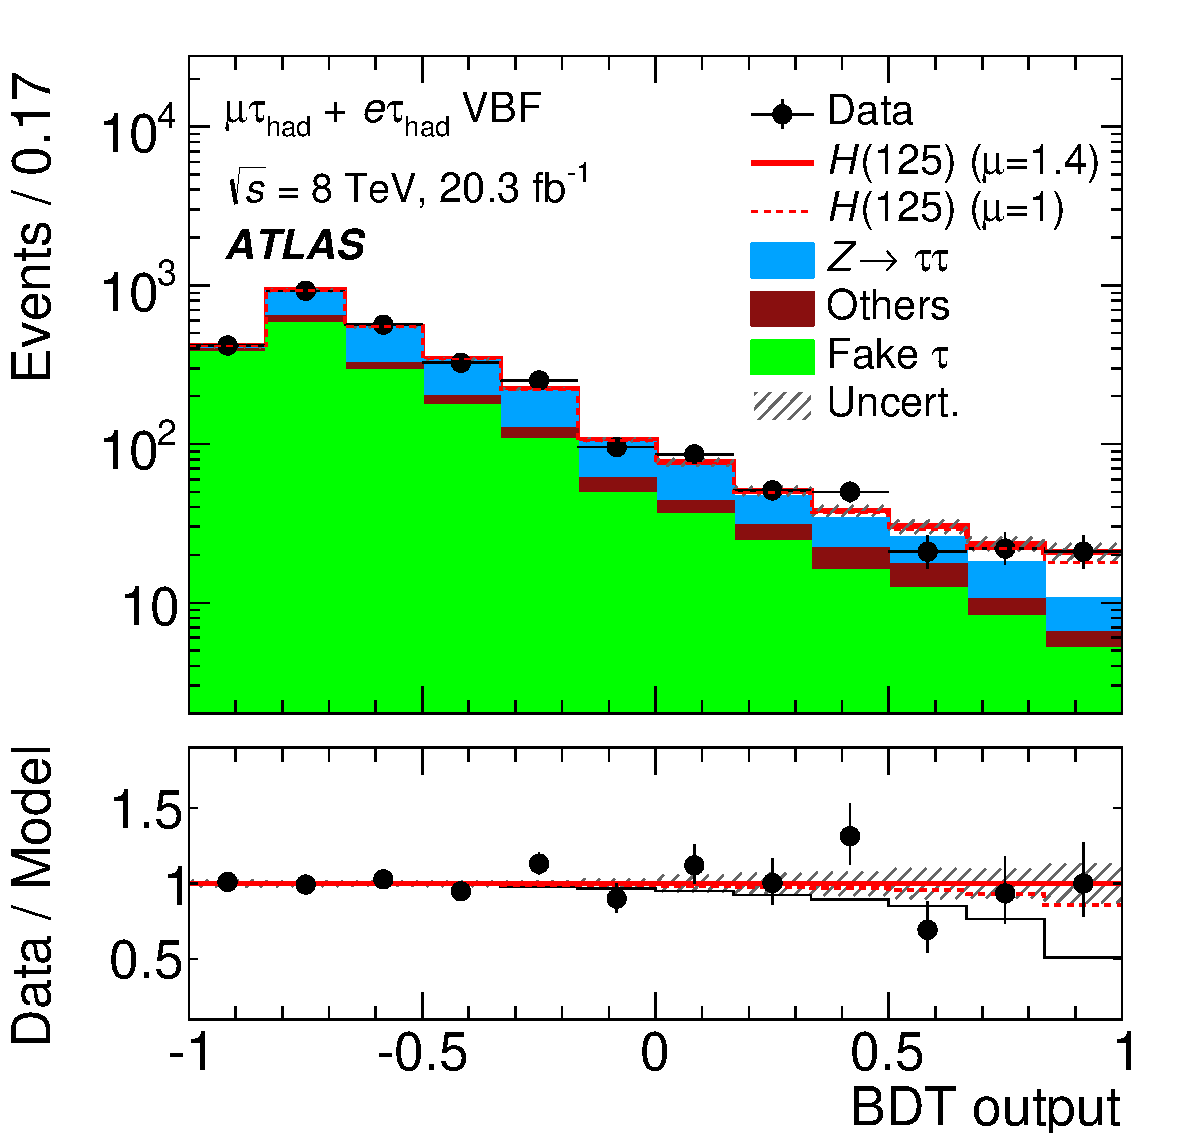
\includegraphics[width=0.48\textwidth]{figures/HIGG-2013-32/fig_08c}
  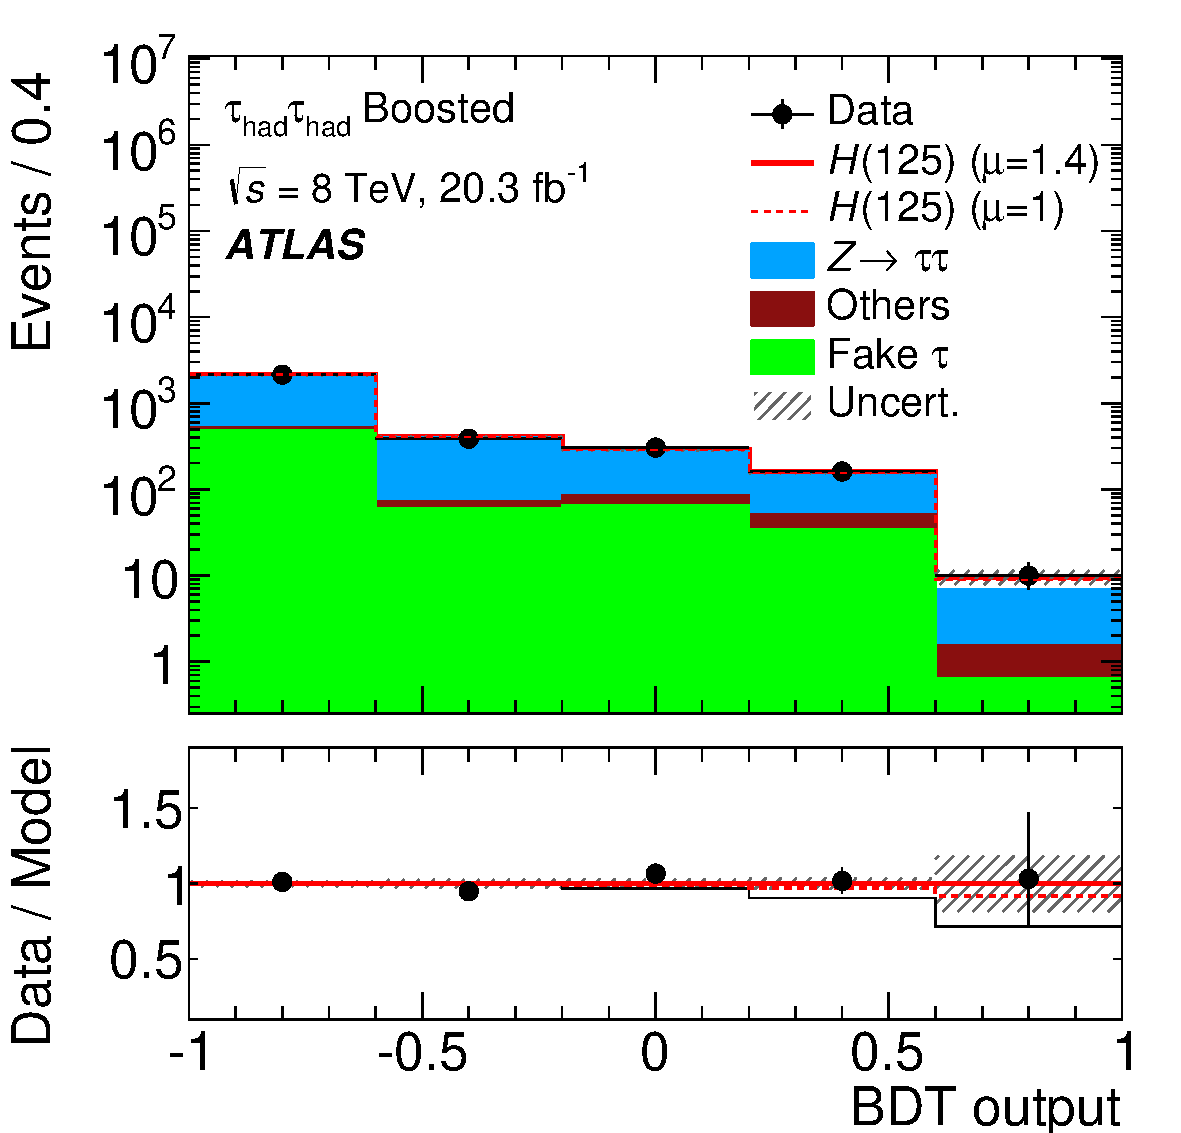
\includegraphics[width=0.48\textwidth]{figures/HIGG-2013-32/fig_08f}
  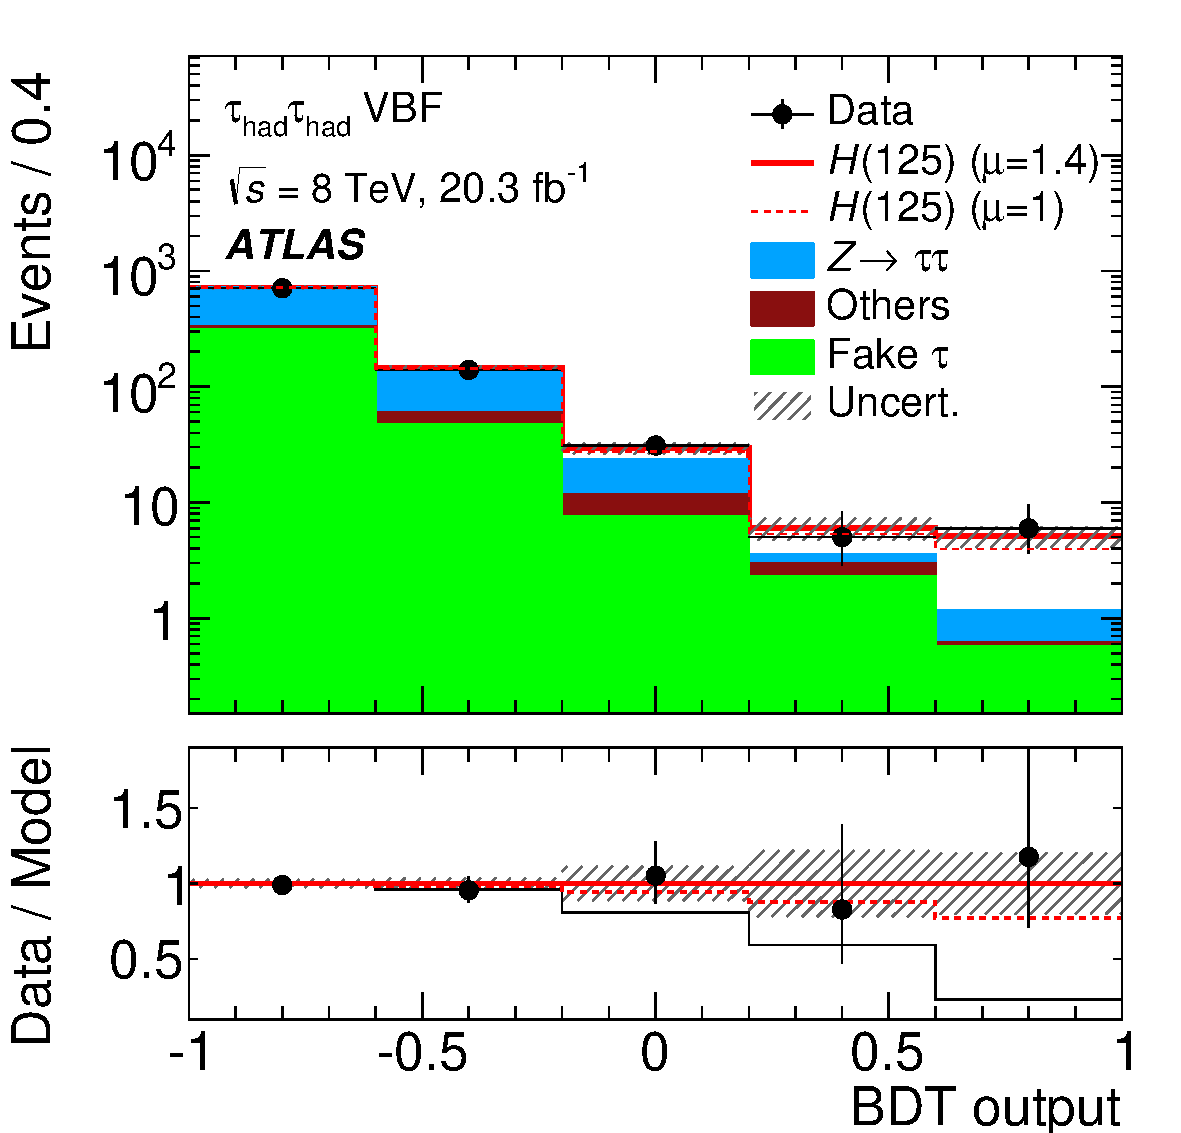
\includegraphics[width=0.48\textwidth]{figures/HIGG-2013-32/fig_08e}
  \caption{Variables.}
  \label{fig:results-bdts}
\end{figure}

\clearpage

\begin{figure}[tp]
  \centering
  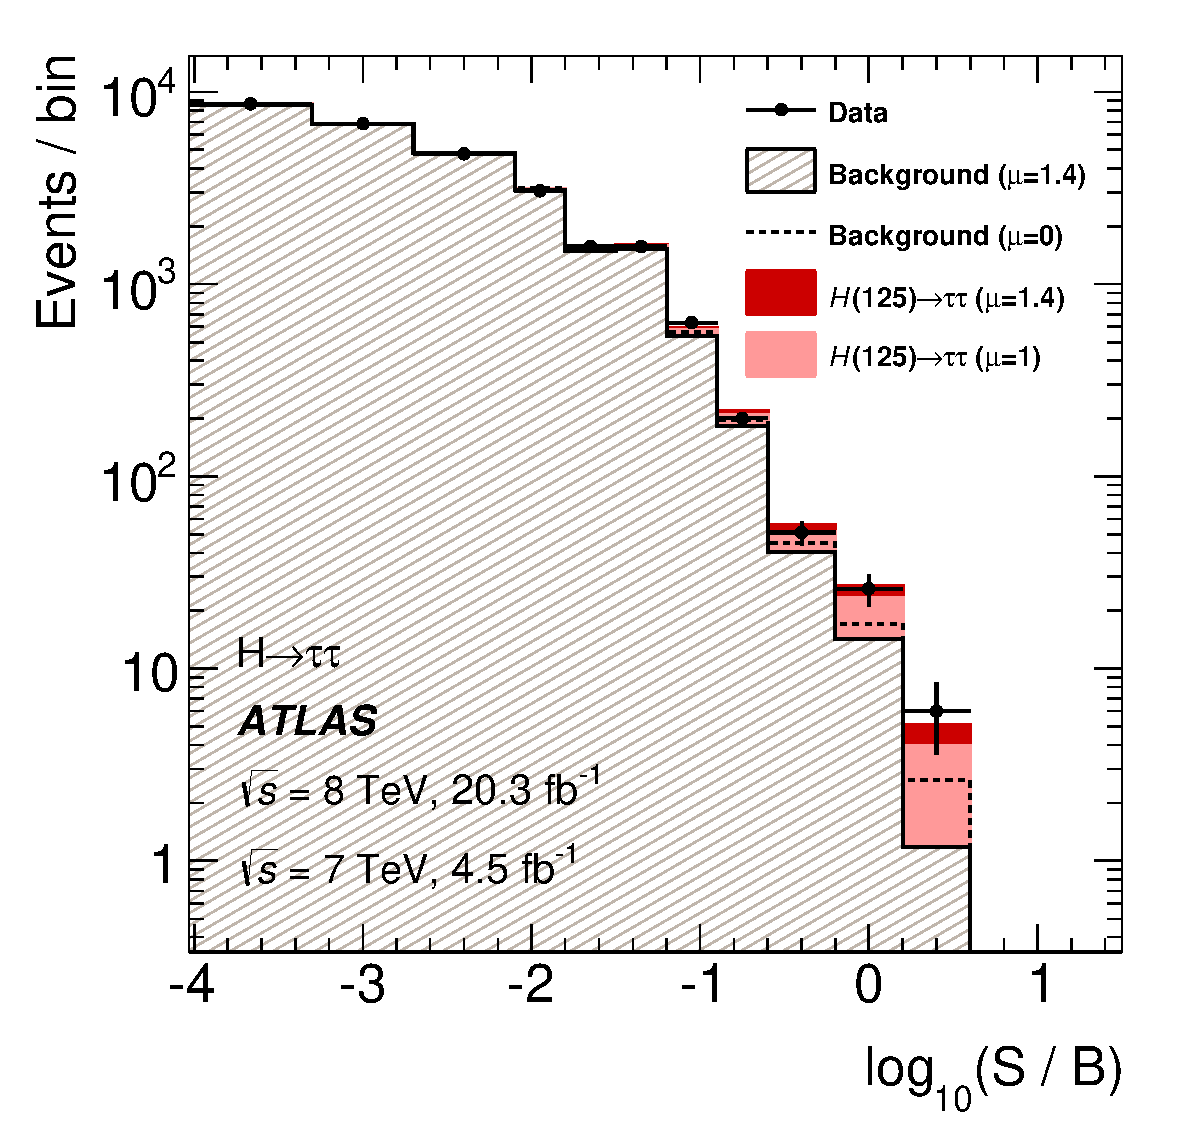
\includegraphics[width=0.48\textwidth]{figures/HIGG-2013-32/fig_10}
  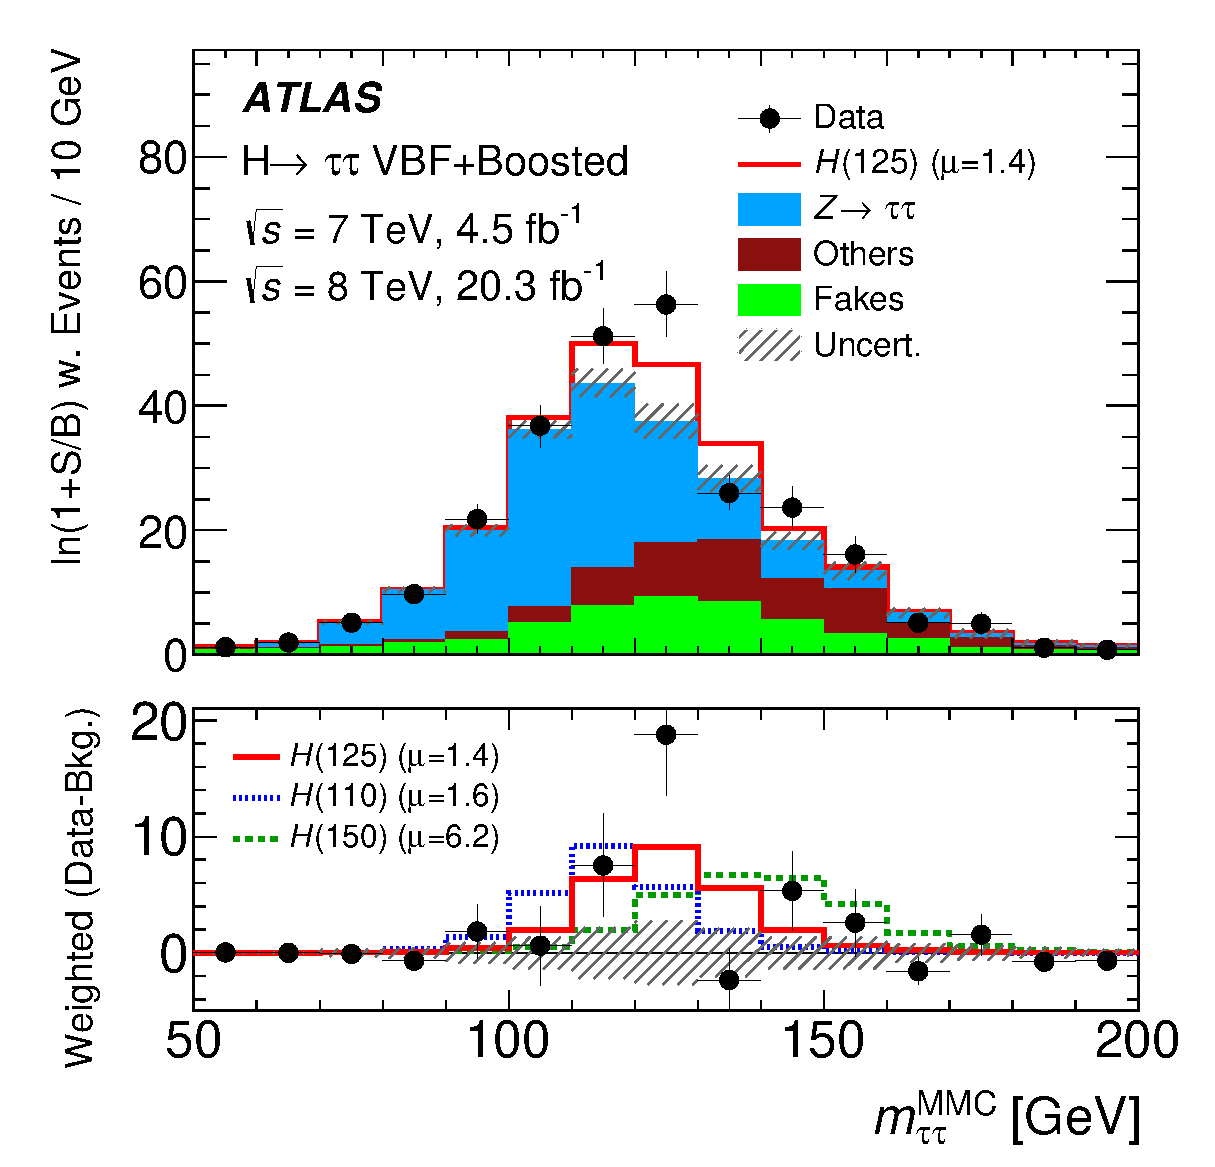
\includegraphics[width=0.48\textwidth]{figures/HIGG-2013-32/fig_11b}
  \caption{Variables.}
  \label{fig:results-money-plots}
\end{figure}

\begin{figure}[tp]
  \centering
  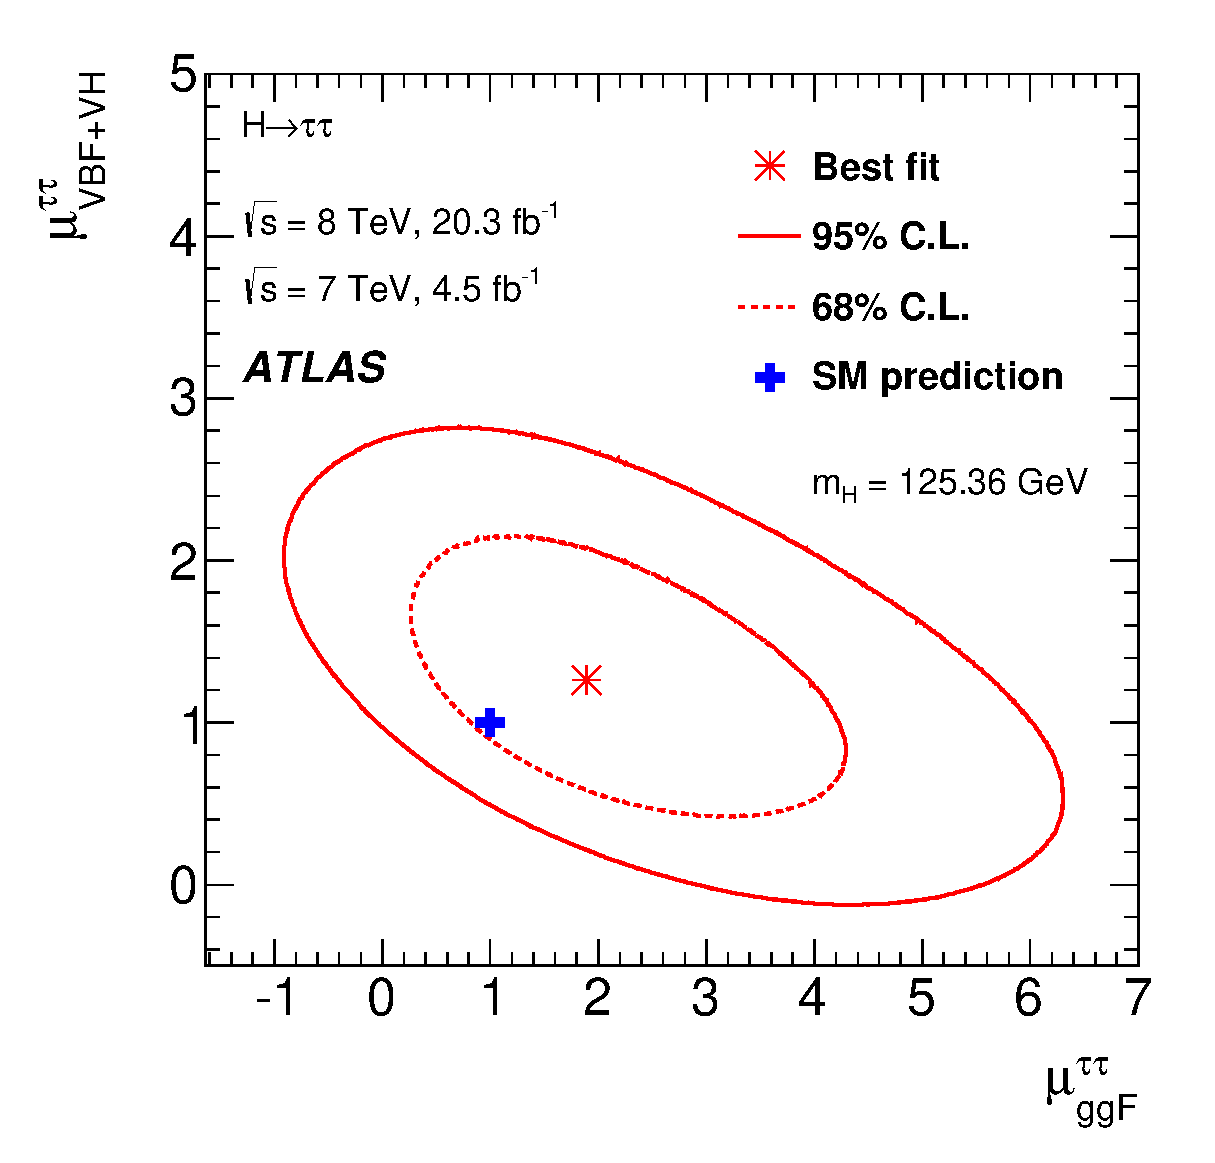
\includegraphics[width=0.48\textwidth]{figures/HIGG-2013-32/fig_12}
  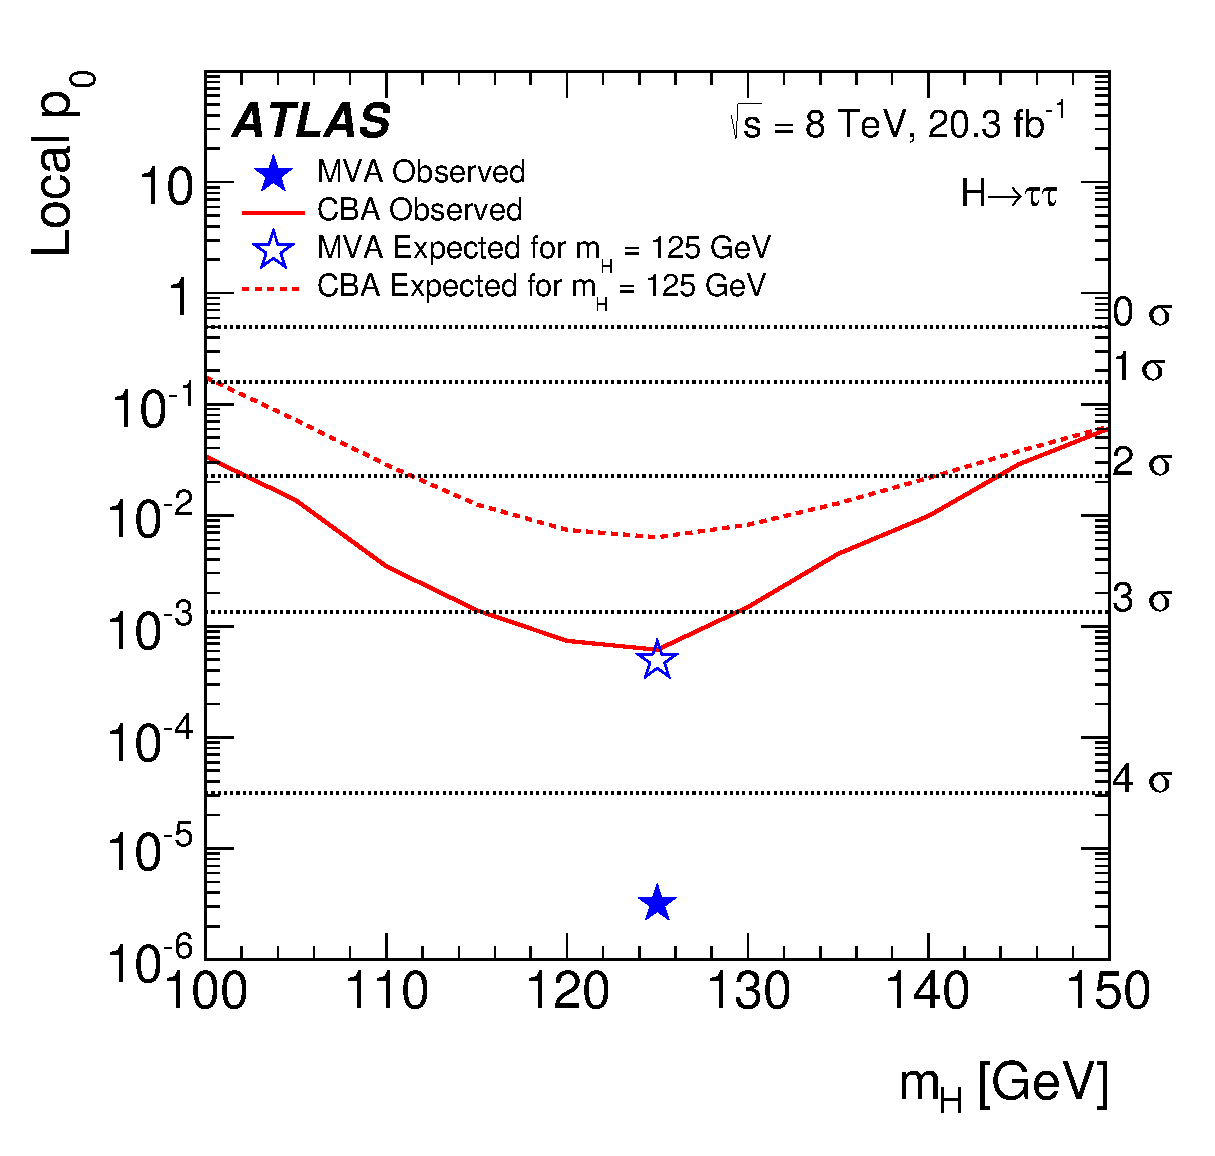
\includegraphics[width=0.48\textwidth]{figures/HIGG-2013-32/fig_14}
  \caption{Variables.}
  \label{fig:results-mup0}
\end{figure}

\begin{figure}[tp]
  \centering
  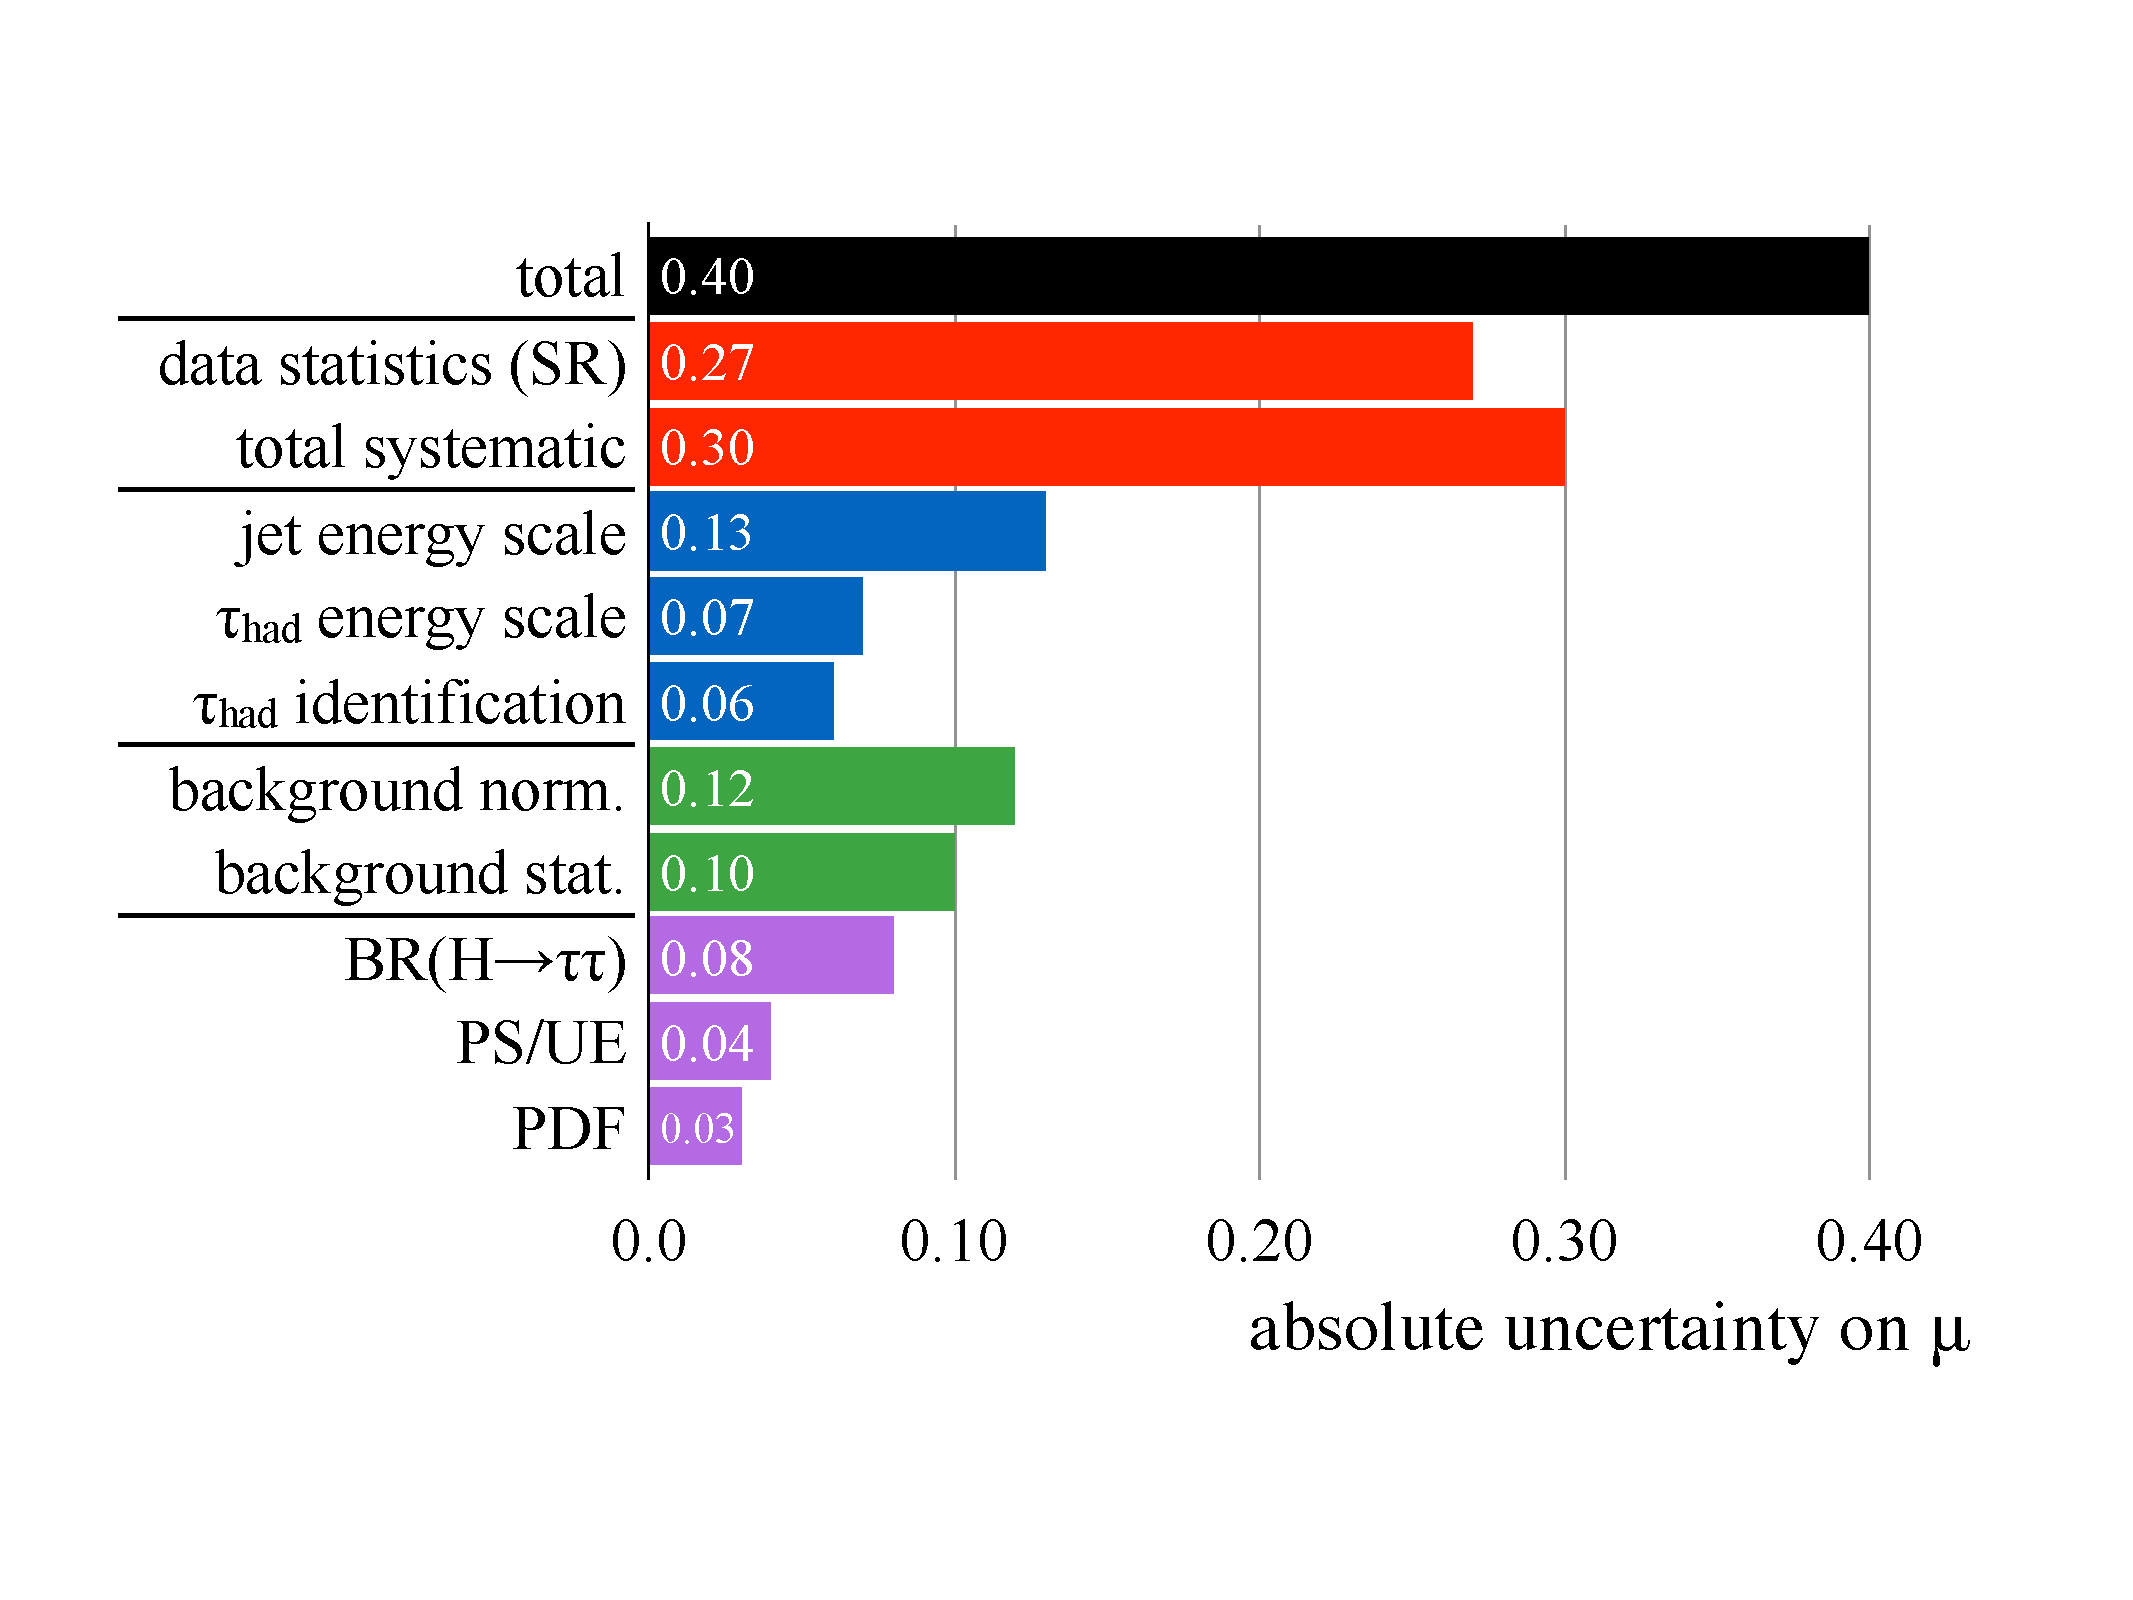
\includegraphics[width=0.90\textwidth]{figures/HIGG-2013-32/uncertainties}
  \caption{Variables.}
  \label{fig:results-uncertainties-1}
\end{figure}

\clearpage
\begin{figure}[tp]
  \centering
  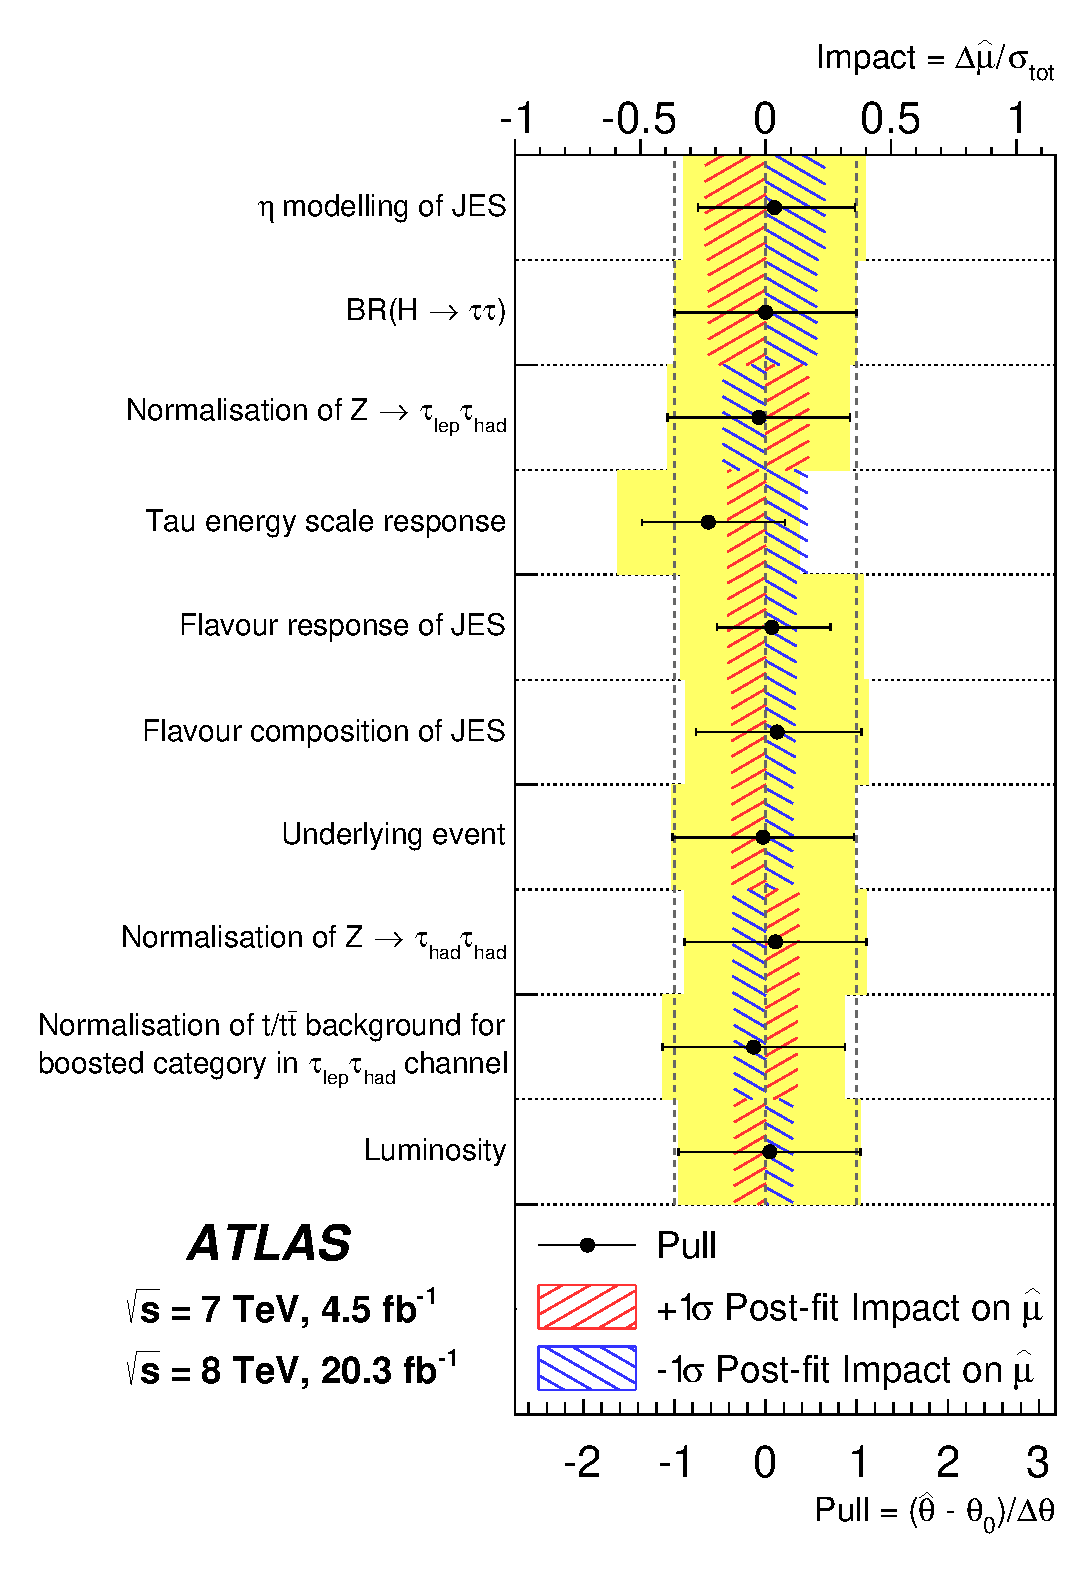
\includegraphics[width=0.90\textwidth]{figures/HIGG-2013-32/fig_07}
  \caption{Variables.}
  \label{fig:results-uncertainties-2}
\end{figure}

\clearpage
\begin{figure}[tp]
  \centering
  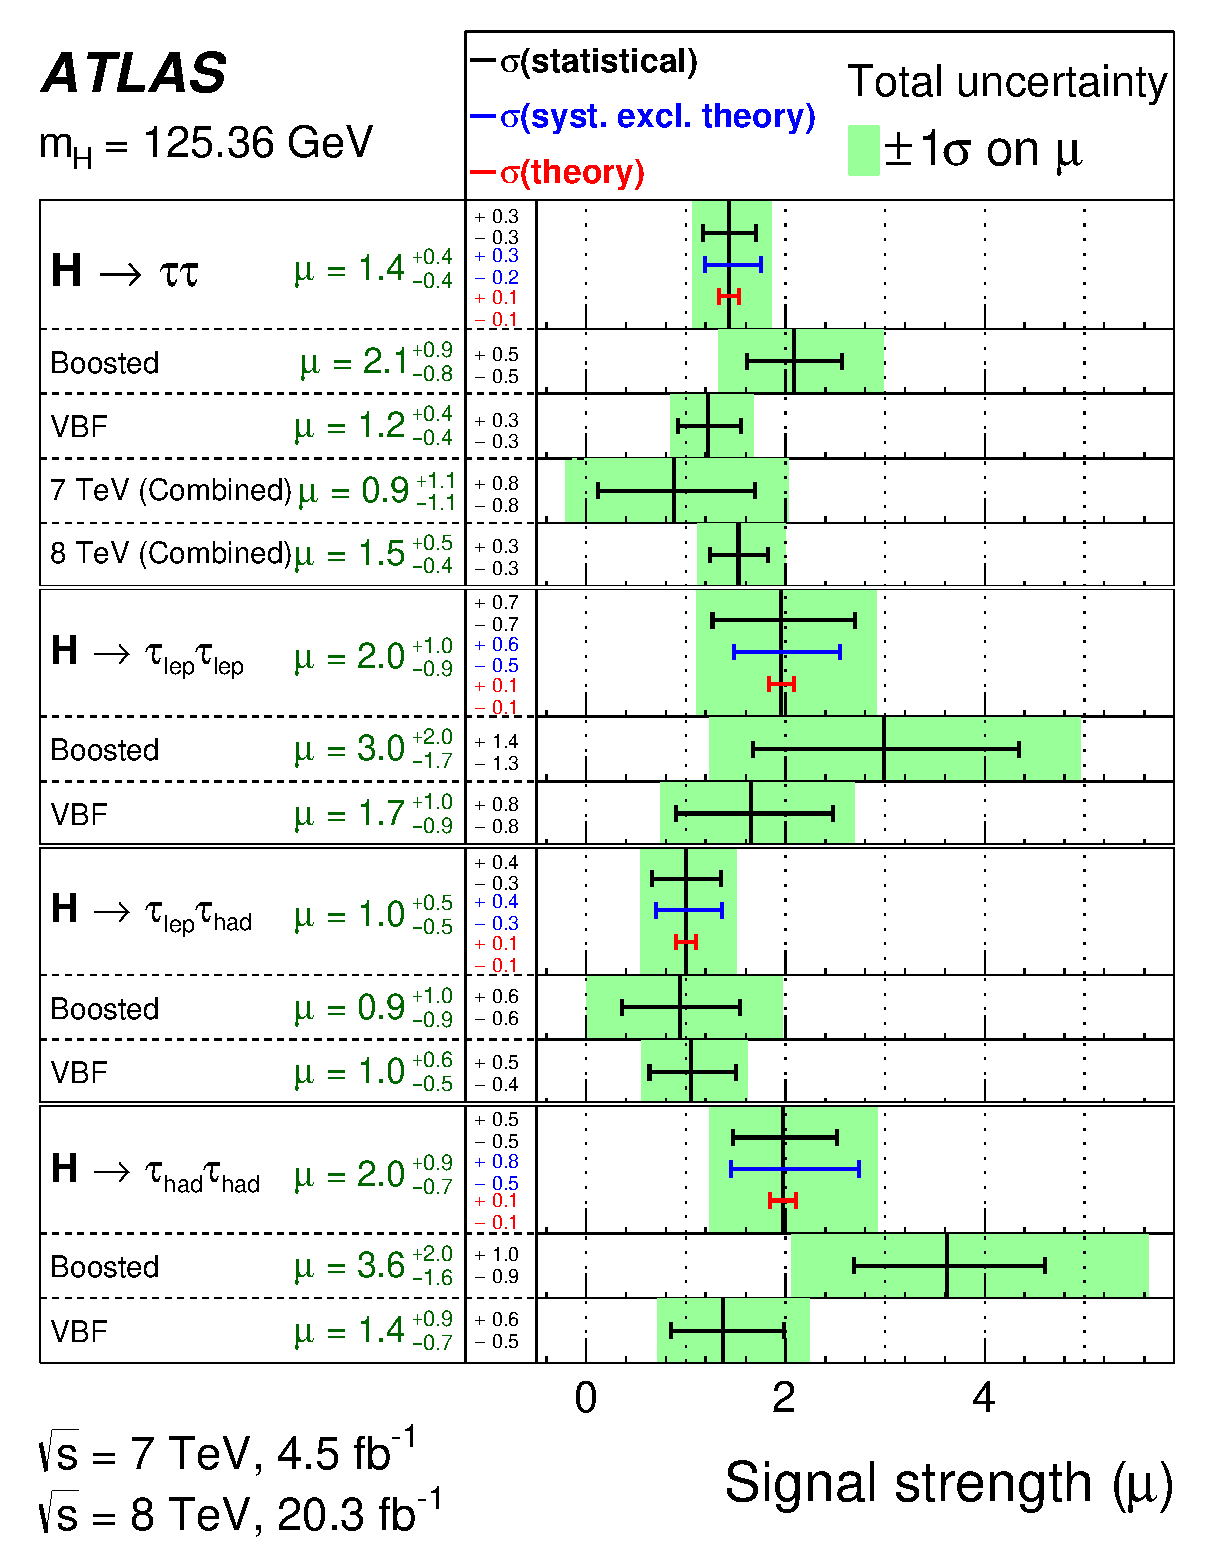
\includegraphics[width=0.90\textwidth]{figures/HIGG-2013-32/fig_09}
  \caption{Variables.}
  \label{fig:results-musummary}
\end{figure}


